\documentclass[tikz,border=2pt]{standalone}
\usepackage{xcolor}
\usepackage{pgfplots}
\usetikzlibrary{arrows.meta}

\pgfplotsset{compat=1.16}
\pgfplotsset{
  singlebarlegend/.style={
    legend image code/.code={
      \draw[##1] (0cm,-0.08cm) rectangle (0.25cm,0.08cm);
    }
  }
}

\definecolor{paperBlue}{RGB}{55,96,146}
\definecolor{paperTeal}{RGB}{74,135,126}
\definecolor{paperGold}{RGB}{190,137,48}
\definecolor{paperRed}{RGB}{164,78,76}
\definecolor{paperGray}{RGB}{92,92,92}

\begin{document}
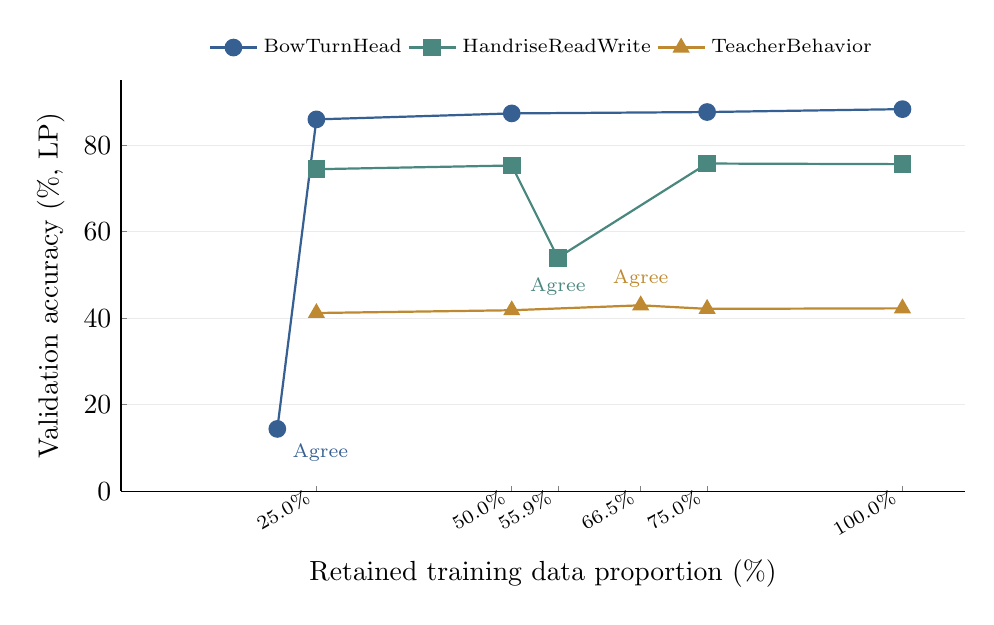
\begin{tikzpicture}
\begin{axis}[
  width=12.3cm,
  height=6.8cm,
  xlabel={Retained training data proportion (\%)},
  ylabel={Validation accuracy (\%, LP)},
  xmin=0, xmax=108,
  ymin=0, ymax=95,
  xtick={25, 50, 55.9, 66.5, 75, 100},
  xticklabels={25.0\%, 50.0\%, 55.9\%, 66.5\%, 75.0\%, 100.0\%},
  x tick label style={font=\scriptsize, rotate=30, anchor=east},
  axis x line*=bottom,
  axis y line*=left,
  ymajorgrids=true,
  grid style={draw=black!8},
  major tick length=2pt,
  legend style={at={(0.5,1.03)}, anchor=south, legend columns=3,
                font=\scriptsize, draw=none},
  mark size=2.8pt,
]
\addplot+[mark=*, thick, color=paperBlue,
          mark options={fill=paperBlue}] coordinates {
  (20.0,14.39)
  (25.0,85.96)
  (50.0,87.34)
  (75.0,87.66)
  (100.0,88.33)
};
\addlegendentry{BowTurnHead}

\addplot+[mark=square*, thick, color=paperTeal,
          mark options={fill=paperTeal}] coordinates {
  (25.0,74.44)
  (50.0,75.30)
  (55.9,53.98)
  (75.0,75.75)
  (100.0,75.61)
};
\addlegendentry{HandriseReadWrite}

\addplot+[mark=triangle*, thick, color=paperGold,
          mark options={fill=paperGold}] coordinates {
  (25.0,41.19)
  (50.0,41.83)
  (66.5,42.97)
  (75.0,42.15)
  (100.0,42.27)
};
\addlegendentry{TeacherBehavior}

\node[font=\scriptsize, paperBlue, anchor=north west, xshift=2pt, yshift=-2pt]
  at (axis cs:20.0,14.39) {Agree};

\node[font=\scriptsize, paperTeal, anchor=north, yshift=-4pt]
  at (axis cs:55.9,53.98) {Agree};

\node[font=\scriptsize, paperGold, anchor=south, yshift=3pt]
  at (axis cs:66.5,42.97) {Agree};
\end{axis}
\end{tikzpicture}
\end{document}